\chapter {Protocole Expérimental}

\section{Matériel utilisé}
En ce que concerne les aspects matériels, le robot bimoteur Wifibot v2, équipé d'un ordinateur à bord, sera utilisé comme plateforme mobile. L'acquisition des données est faite par une camera RGB-D Asus Xtion Pro Live. Par rapport au choix logiciel, l'environnement robotique ROS\footnote{Robot Operating System} a été adopté pour avoir les bibliothèques qui permettent de gérer les nuages de points, Freenect, OpenNi2 et PCL\footnote{Point Cloud Library}, et d'autres nombreux outils de contrôle du robot et sauvegarde d'informations.

\section{Setup expérimental}
Pour évaluer les capacités de reconnaissance du robot, vingt objets de tailles et formes diverses ont été choisis pour être incorporé à la base de connaissance. Ils s'agit d'objets typiques qui peuvent être facilement retrouvés dans un laboratoire ou un bureau. Ensuite, nous avons effectué un tour complet de l'objet avec le robot en sauvegardant les nuage de point et en extrayant les features VFH pour huit positions différentes écartées de 45 degrés à 1.5 mètres de distance. La position correspondent à l'angle zéro a été choisie de manière aléatoire en alignant un des axes de l'objet avec celui du capteur. L'image \ref{fig:setup_expe} des vues d'un objet exemplifie la composition de la base de données. Une liste complète des objets figure en annexe \ref{fig:dataset}.

\begin{figure}[H]
	\subfloat{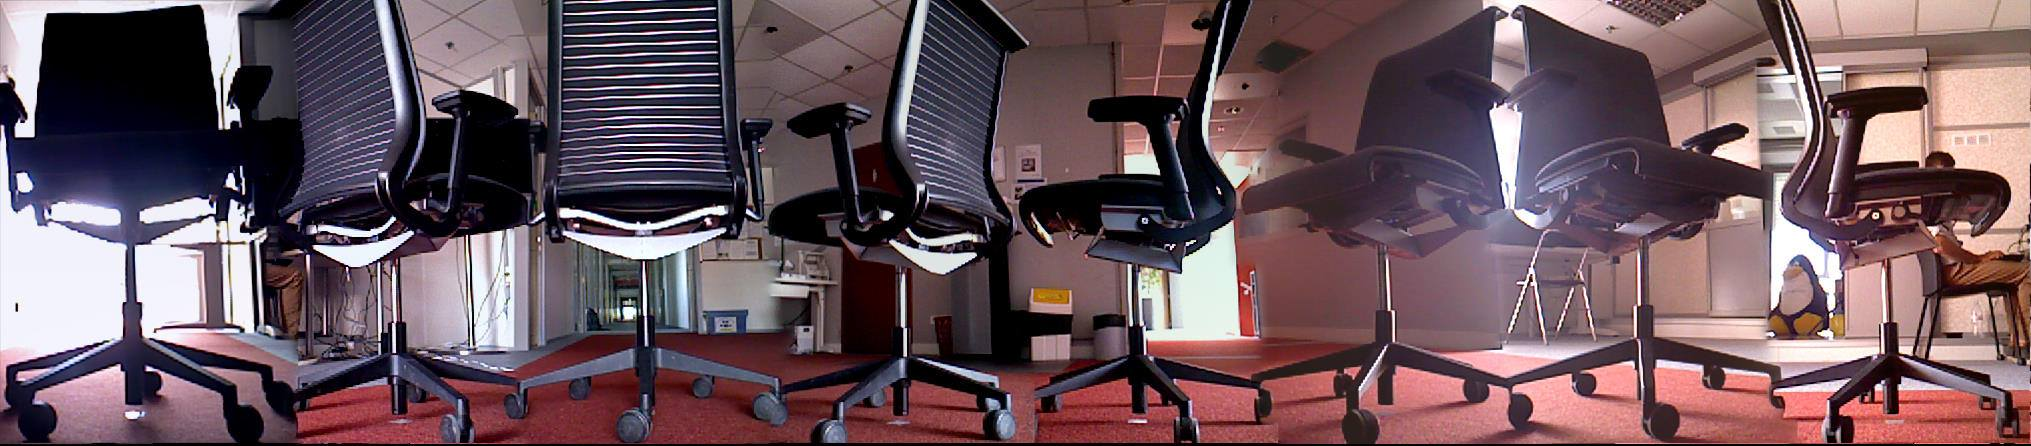
\includegraphics[width=\textwidth]{chair_db.jpg}}		
	\caption{Les huit point de vues de l'objet commençant par la position zéro et en tournant le robot en sens horaire}
	\label{fig:setup_expe}
\end{figure}

\section{Résultats expérimentaux}
\subsection{Comparaison à la reconnaissance mono-vue}
Une première évaluation consiste à faire un tour complet autour de l'objet à reconnaitre pour quatre positions angulaires différentes : $0, 45, 90$ et une dernière choisie de manière aléatoire pour chaque objet. Le robot fait le tour à une vitesse de $0.35 \pm 0.1 m/s$ à une distance de $1.5m$, en enregistrant des images à $1hz$, ansi, une expérience typique est constituée d'environ $25$  images d'angle différent et prendre $25 \pm 3$ seconds. 

La difficulté de l'évaluation vient, premièrement, du fait du robot avoir une base assez discrète ce qui donne marge à des mauvaise reconnaissance mono-vue une fois le point de vue étant inexistant dans la base de connaissance. Puis, la vitesse du déplacement résulte dans images plus floues lors des acquisitions et la modification de l'angle de la caméra\footnote{L'angle entre la base et la tête de la caméra Asus Xtion est facilement modifié.} apportent un obstacle en plus pour le \textit{matching} de descripteurs dans le classificateur K-plus proches voisins.

Un expérience typique est illustrée dans l'image \ref{fig:resultats_expe} :

\begin{figure}[H]
	\subfloat{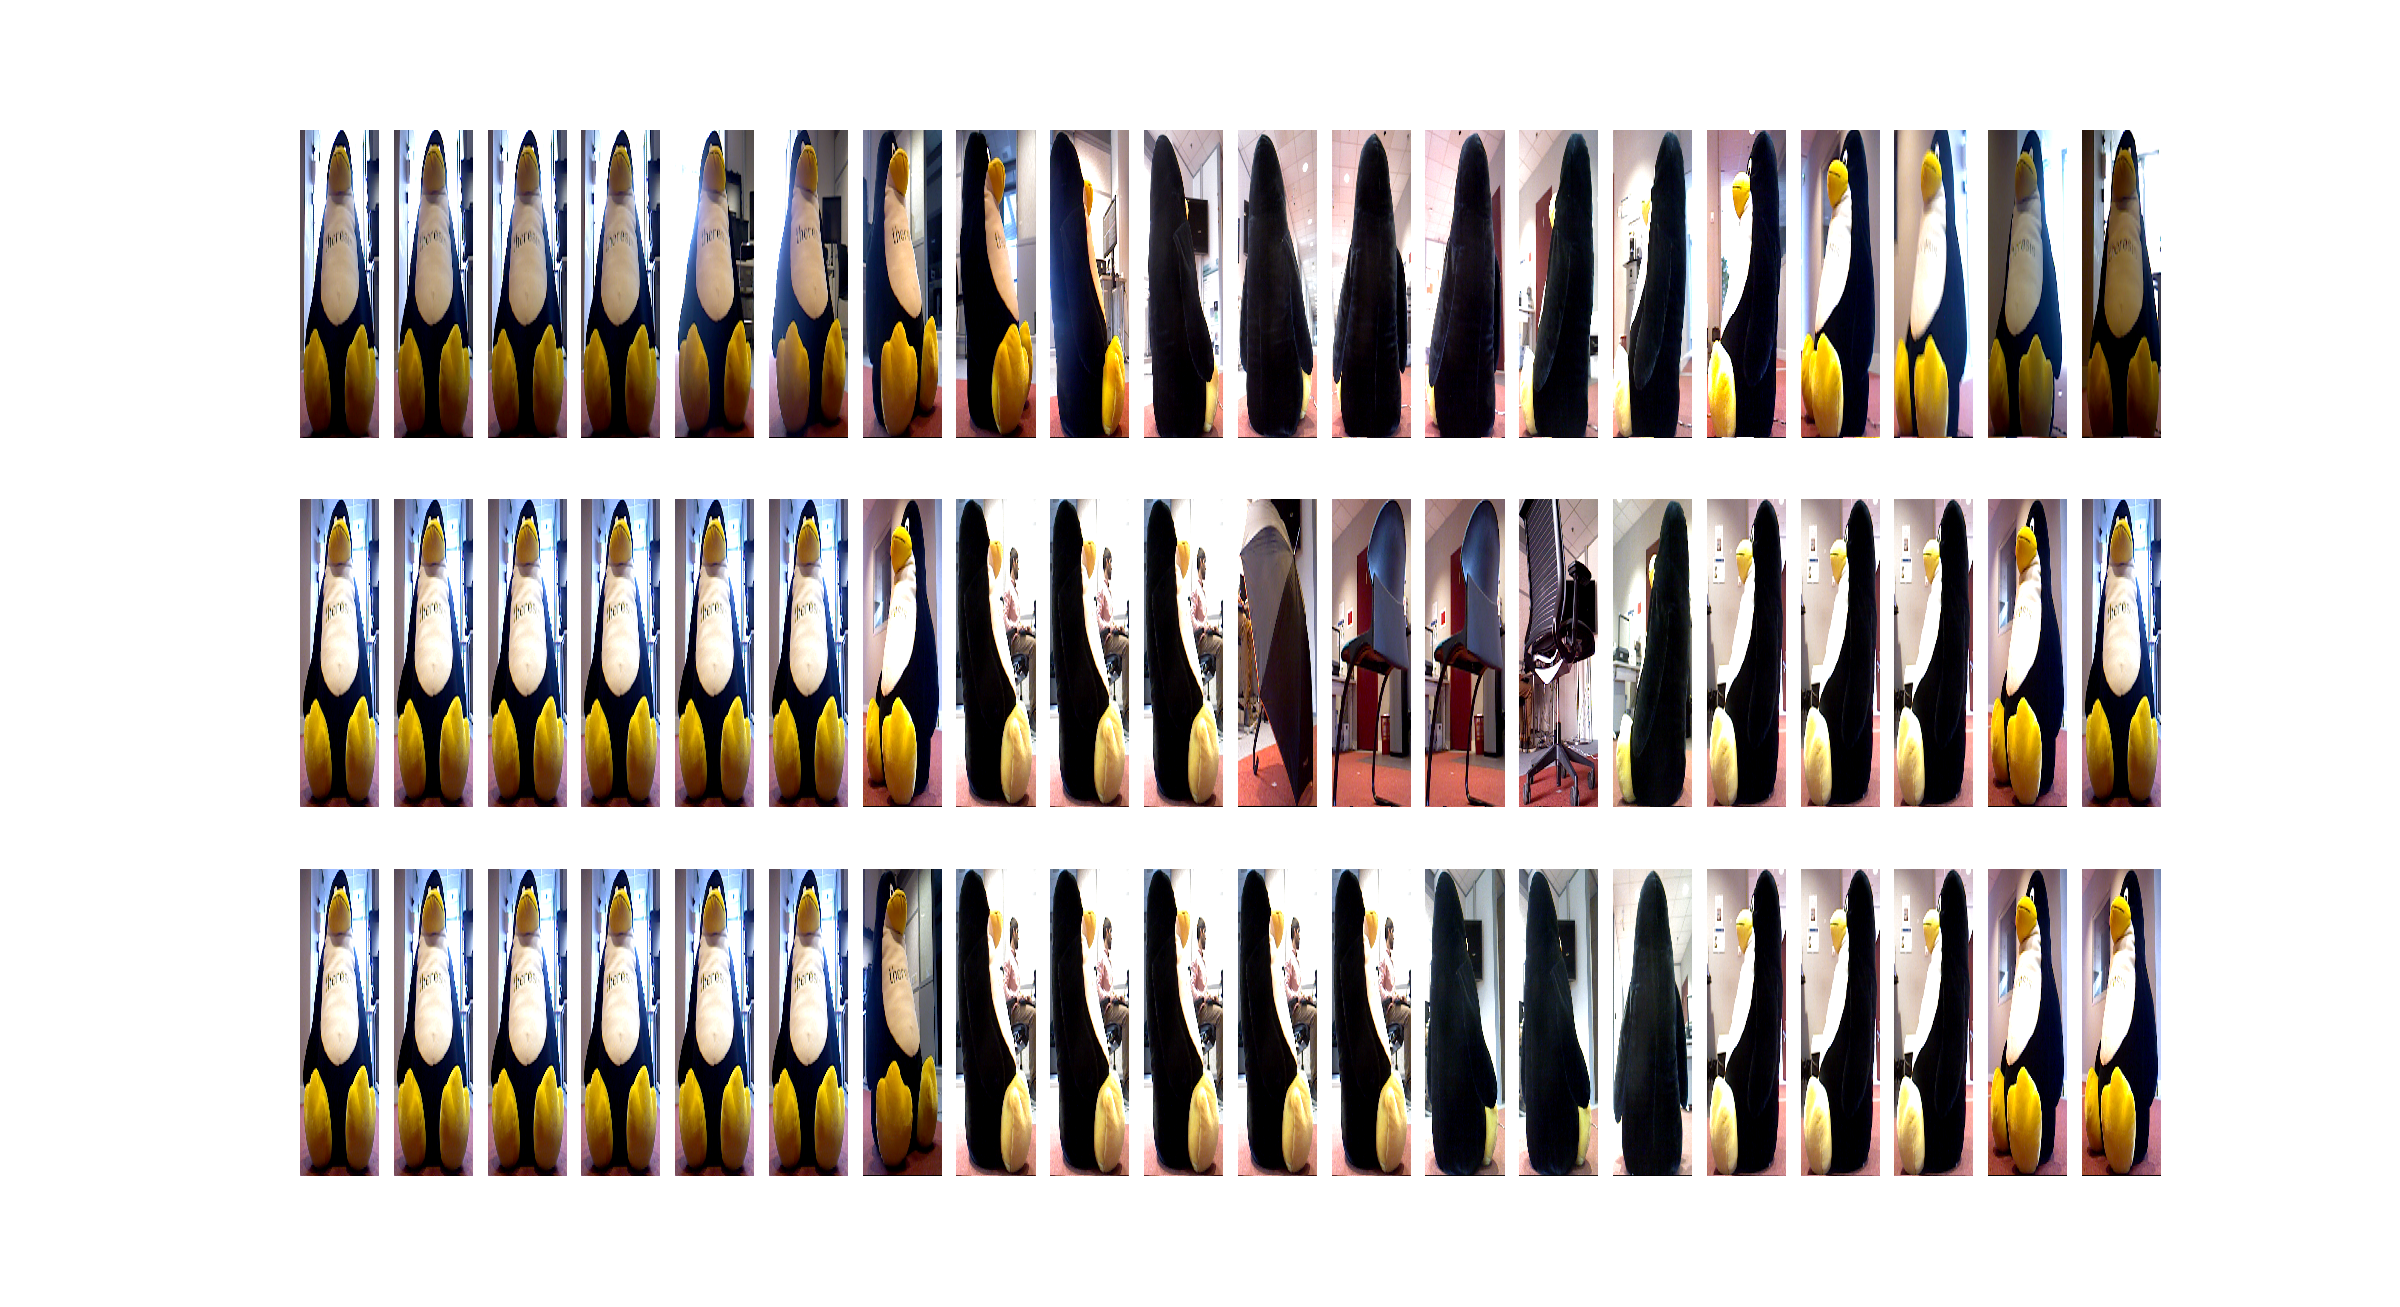
\includegraphics[width=\textwidth]{hmm_example.png}}	
			\caption{\textbf{Résultat de l'évaluation} - Reconnaissance multi-vue corrige des ambiguïtés et surmonte la mauvaise segmentation lors de la création de la base.}
	\label{fig:resultats_expe}
\end{figure}

La première ligne correspond à la séquence d'images vues par le robot à chaque instant de temps, et donc, l'objet à être reconnu. La seconde ligne, donnée par l'algorithme de reconnaissance, équivaut à la vue la plus probable de l'objet reconnue par le K-plus proches voisins. Il est intéressant remarquer que l'invariance à rotation du descripteur trompe l'estimation de l'orientation en prenant son correspond énantiomorphe dans le premier carré rouge. Autrement, le dos du pinguin étant une grande surface presque plane, il est partiellement retiré par l'étape de segmentation. Ainsi, le nuage de points résultant de ce point de vue n'est pas suffisamment complet pour caractériser correctement l'objet, ce qui induit une mauvaise reconnaissance dans le carré bleu. Au final, on remarque que le traitement apporté par la chaîne de Markov cachée permet de corriger les problèmes d'une base de donnée relativement sparse avec des possibles erreus de segmentation, permettant la correction simultanée de la reconnaissance de l'objet et de son orientation en ligne. 

%\begin{figure}[H]
%	\subfloat{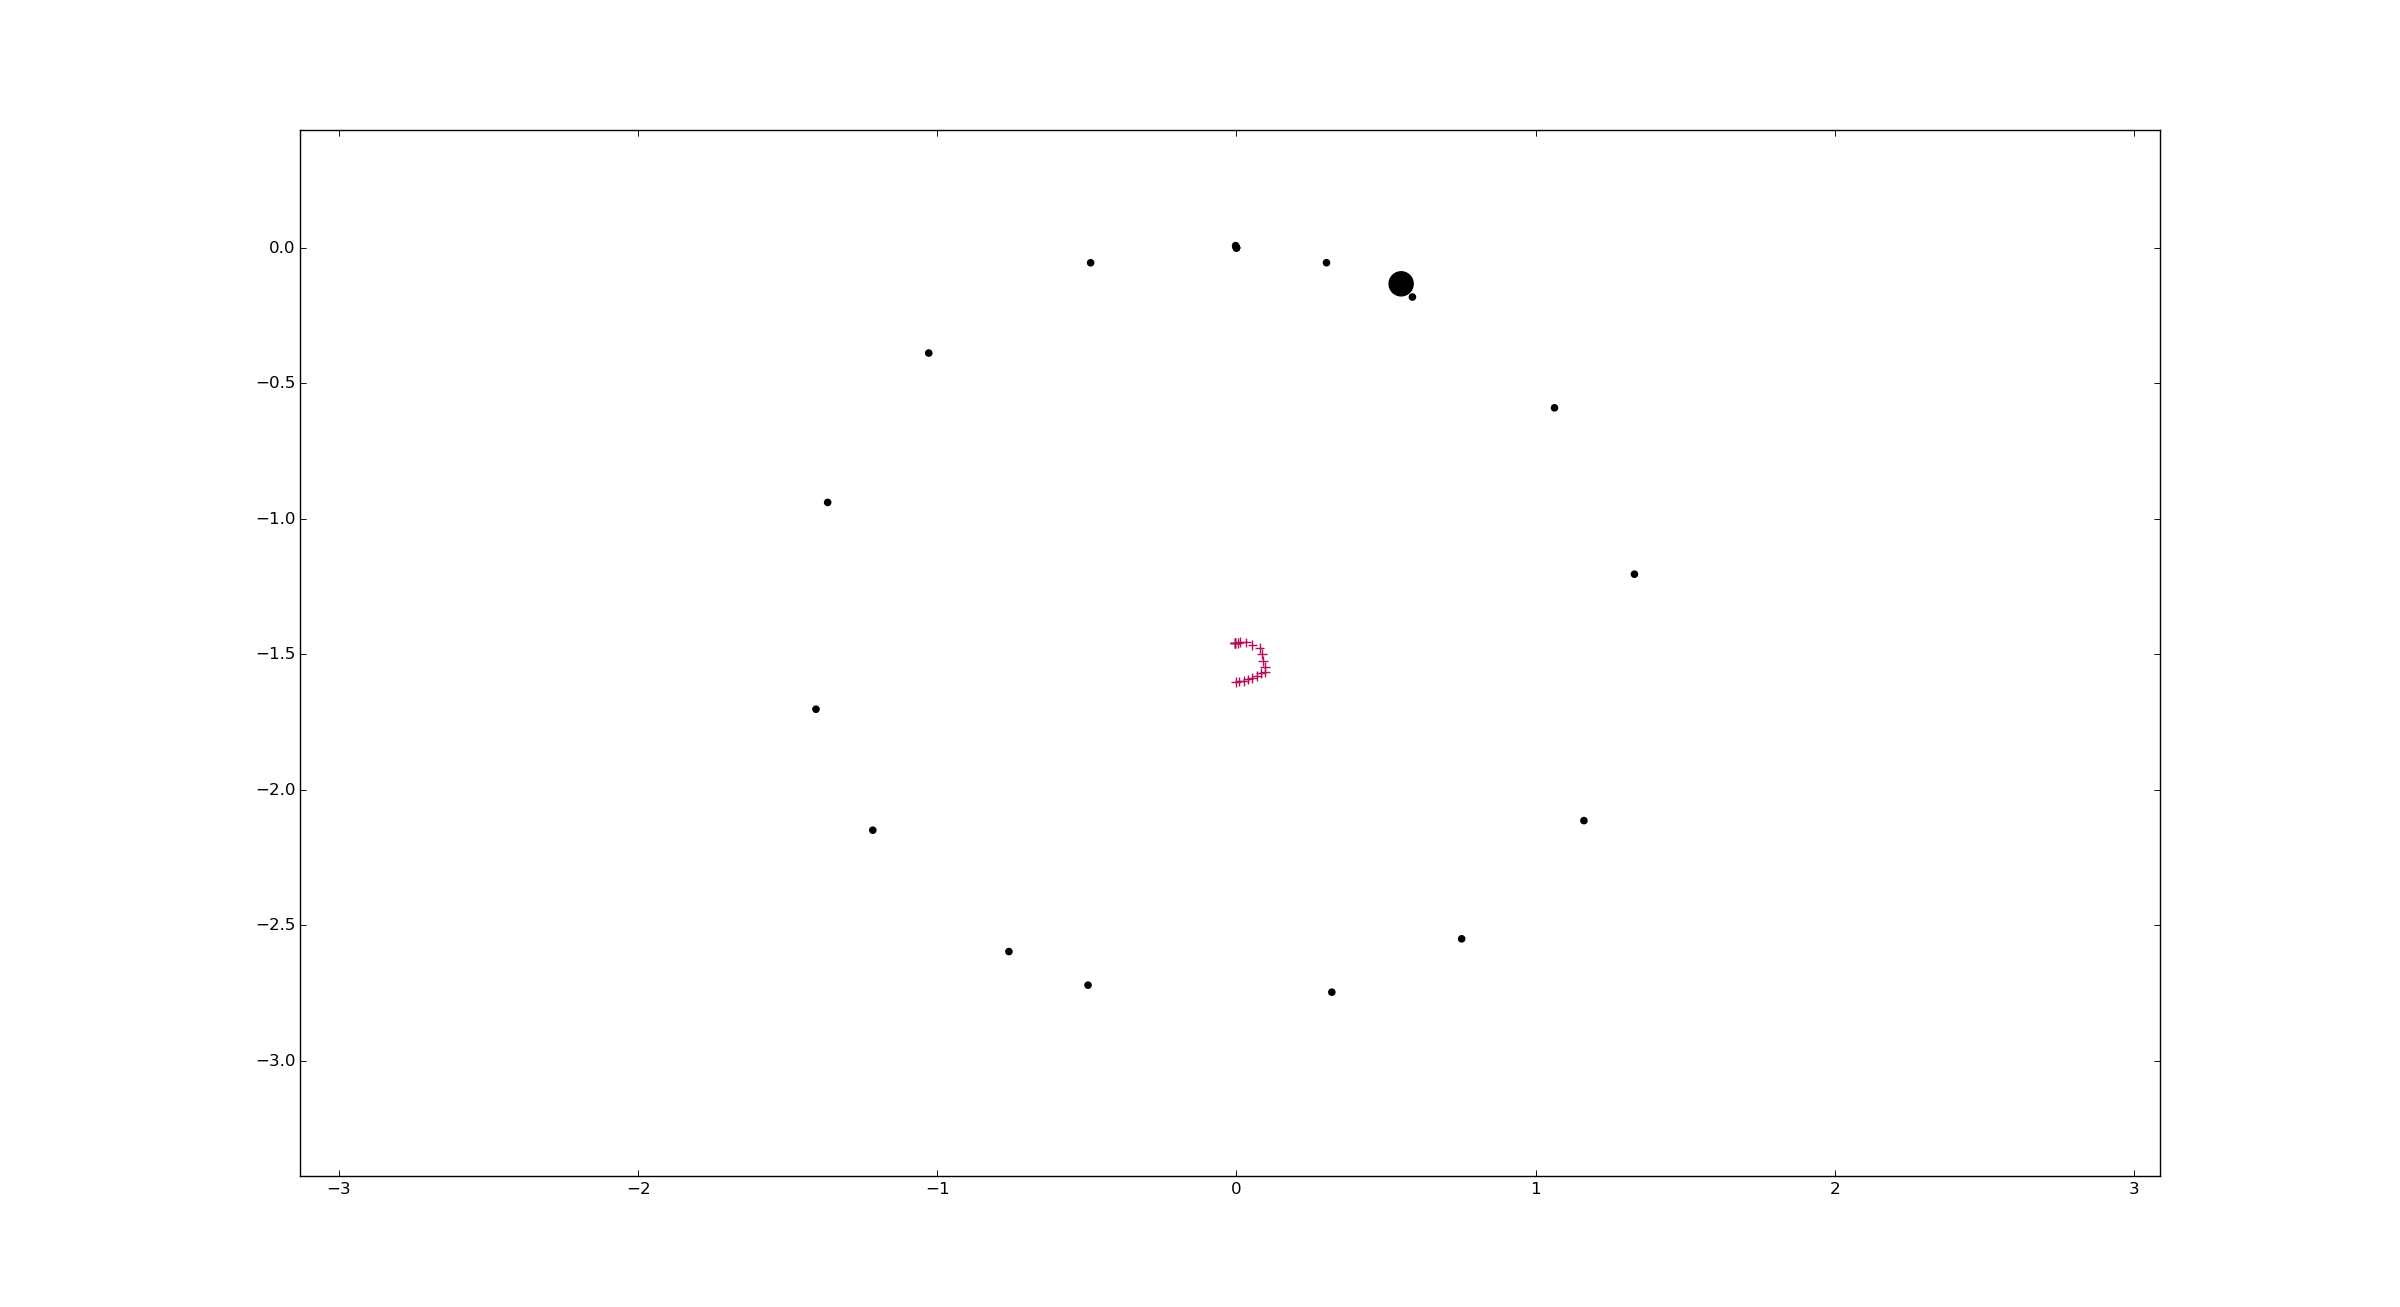
\includegraphics[width=\textwidth]{hmm_mov.png}}		
%\end{figure}


{\color{green}
Dans le premier tableaux on retrouve le résultats de la reconnaissance donné par la comparaison des histogrammes provenant du *plus proche voisin*. Ce résultat estime la capacité de distinguer deux objets quelconques, en autre mots, cette capacité viens de la représentativité des descripteurs utilisés et l'efficacité de la mesure de similarité entre histogrammes.
}

%\subsection{Robustesse à l'occlusion}

\subsection{Suivi et reconnaissance multi-cibles}

Le deuxième expérimentent correspond à placer des objets appris auparavant dans une pièce et conduire le robot faisant en sort qu'il les regardait de plusieurs points de vues différents. 
Ce scénario est beaucoup plus complexe que celui d'avant. D'abord les objets occultent uns aux autres résultant en mauvaises segmentations. Ensuite, la suivi d'objets est plus complexe
La carte finale donnée par l'algorithme, \ref{fig:multi_map}, 

\begin{figure}[H]
	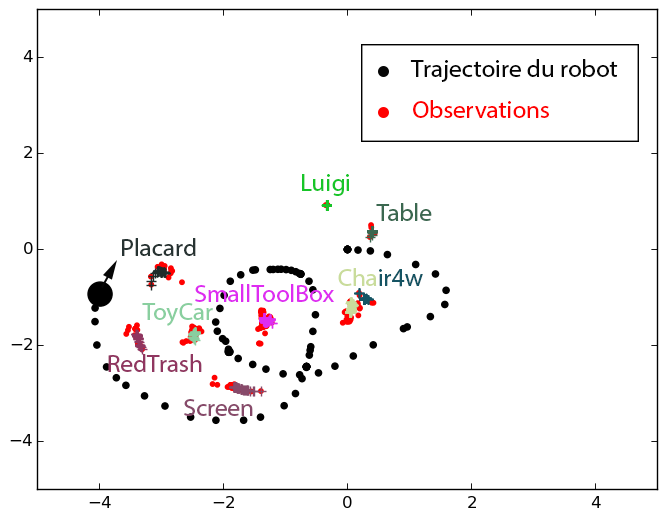
\includegraphics[width=\textwidth]{map.png}
	\caption{...}	
	\label{fig:multi_map}
\end{figure}

\section{Problèmes rencontrés}

\subsubsection{Synchronisation}

\subsubsection{Problèmes de déplacement}

La roulette de support originalement installée avait deux axes de
rotation. Pourtant, quelques mouvements de rotation du robot alignent
la roulette orthogonalement au sens du prochain mouvement ce qui crées
une torche parasite que perturbe la trajectoire voulue. Une tentative
frustrée d'installer une bille omnidirectionnelle à roulement, qui se
bloquait sur la moquette avec le poids du robot, a fait que
l'originale était réinstallée. Une deuxième solution serait d'interdire
certains mouvements du robot pour éviter cette déviation.